\section{Table Segmentation}

The following assumptions were made for the segmentation of the table
\begin{itemize}
    \item the table is a uniform color and is a prevalent part of the image
    \item the table is centered (or close to being centered) in the image
\end{itemize}

It is going to be apparent the reason for these when the full algorithm for
the segmentation of the table is explained.
The first thing that was to be found was a rough segmentation of the table,
as finding the lines with only the Canny-transform of the full image would 
be problematic, as the strongest lines in the image are not only the table
fabric, but also the table itself and various other things in the image.
The initial approach was to use Otsu's thresholding, as the table is a uniform
color, therefore it is sensible to assume it would be thresholded the same
way throughout. This proved unfruitful, as the segmentation was too rough as shown in figure \ref{fig:otsutable}.
The second approach was to use kmeans clustering, in particular exploiting the
adaptability of the algorithm in order to use spatial features too to improve
the segmentation, as we assume the table is a continuous entity. Out of the k clusters obtained the most centered one was picked as shown in figure \ref{fig:kmeanstabol}.
The segmentation obtained was fairly precise but contained multiple disconnected
components, however we can consider the table the biggest and pick it, in particular
before doing this, the morphological operation open is applied in order to remove weakly connected objects.
the k (empirically) chosen was 3, as 2 lead to undersegmentation of the image and 4 to oversegmentation.
The resulting segmentation is precise in most cases, but given the nature of kmeans on some
images it fails, as it clusters some unrelated parts of the table with the fabric, due,
for example, to lighting.
For this reason further processing was required: given we have obtained a rough mask of
the table we now obtain the mean color of the image in the pixels where the mask is non-zero.
After this we use a color thresholding by distance, as shown in figure \ref{fig:colorsegtabol} from the mean and the same way we 
did before to obtain the largest connectedcomponent. thresholding on the hue
is the most robust (instead of using the distance between bgr colors), in particular a low distance, 5, was chosen, but different values close to 5 similar results.\par
after having obtained this result dilation is applied in order to remove some noise from the mask,
for example balls or other objects. Afterwards the hough transform is used to find the lines, 
with a threshold in order to remove similar lines.
The vertices of the table are found using the equations from \href{https://en.wikipedia.org/wiki/Line\%E2\%80\%93line\_intersection}{wikipedia}.
It is to note that the last frame is used for such frame as most of the time it doesn't contain the player in the table, being at the end of
a turn.
The segmentation found is technically not precise, we count as part of table player, holes and billiard balls. The last can be easily solved by simply adding back the balls that are detected. 
As for the the other two other cases they are ignored for a compromise in performance, as in some
cases the change in illumination is severe, causing some parts of the table to have extreme 
differences in color, for example the internal parts of the table. It is also to consider that the morphological operations used to isolate the connected component of the table will also worsen
the general outlines. For this reason the output of the line detection is preferred, as it yields
more consistent and stable results, as shown in figure \ref{fig:finalsegtabol}.

\begin{figure}[h!]
    \centering
    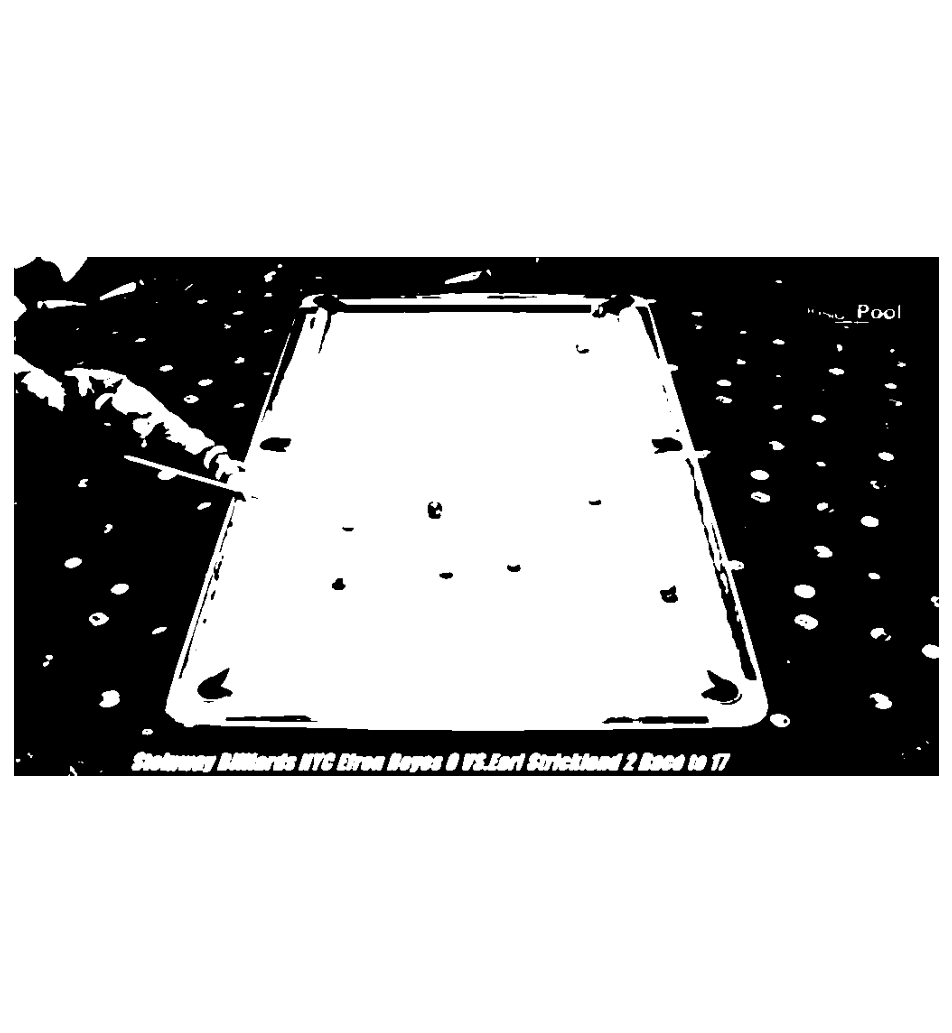
\includegraphics[width=0.4\textwidth]{./imgs/otsu_table.png}
    \caption{Example of Otsu Segmentation}
    \label{fig:otsutable}
\end{figure}

\begin{figure}[h]
    \centering
    \begin{subfigure}[b]{0.75\textwidth}
        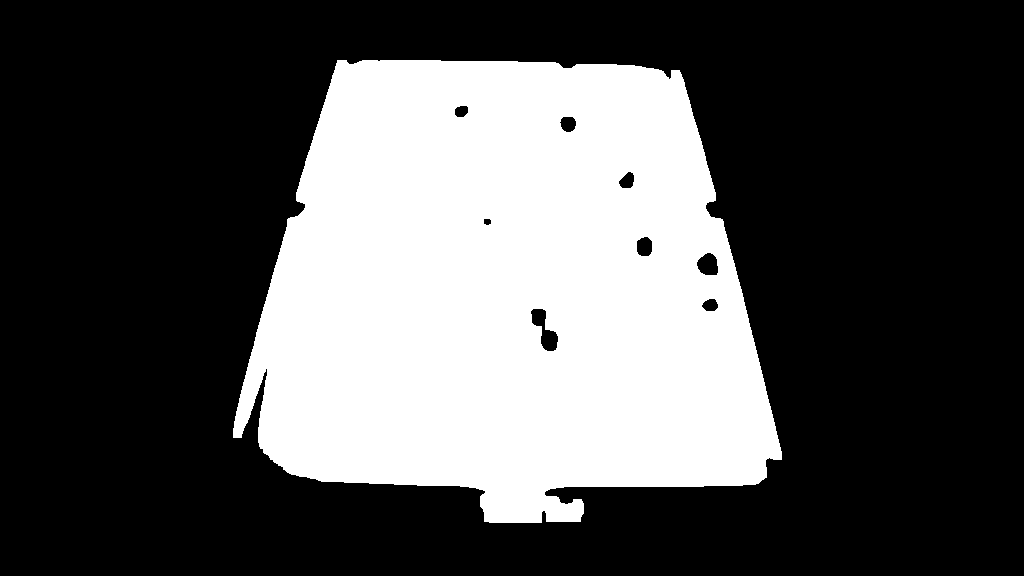
\includegraphics[width=\textwidth]{./imgs/kmeans_cluster.png}
        \caption{Initial kmeans clustering result}
        \label{fig:kmeanstabol}
    \end{subfigure}
    \\
    \begin{subfigure}[b]{0.75\textwidth}
        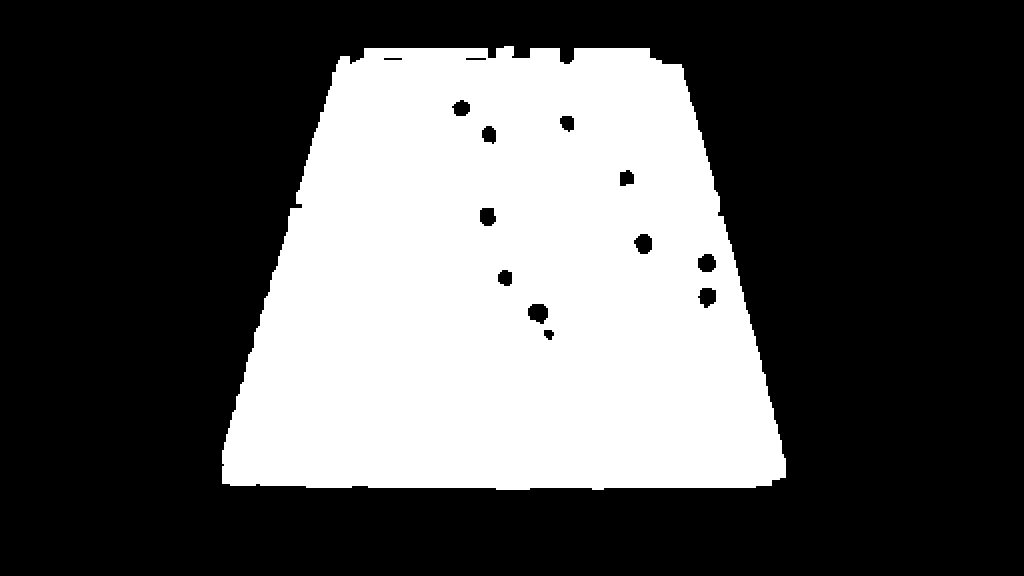
\includegraphics[width=\textwidth]{./imgs/color_cluster.png}
        \caption{Color clustering result}
        \label{fig:colorsegtabol}
    \end{subfigure}
    \\
    \begin{subfigure}[b]{0.75\textwidth}
        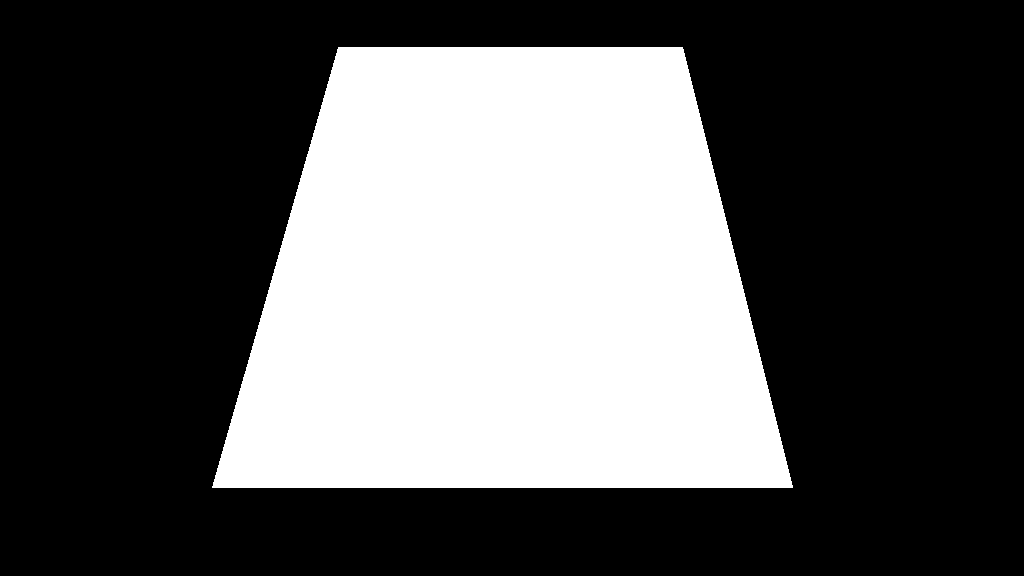
\includegraphics[width=\textwidth]{./imgs/maskfill.png}
        \caption{Mask obtained from filling the area contained in the lines found}
        \label{fig:finalsegtabol}
    \end{subfigure}
    \caption{Stages of the segmentation}
    \vspace{30pt}
\end{figure}
